DDFEM is a combination of embedded finite elements and hierarchical
coarsening.
In this section, we discuss the problem of coarsening
and introduce the notion of a material palette. We conclude by
summarizing the two main stages of DDFEM—offline metamaterial
construction and online coarsening.
\paragraph{Coarsening for finite elements}
The key component of our DDFEM is coarsening.
Coarsening reduces the number of vertices in a finite element simulation mesh in order to improve
runtime performance.
Since simply removing vertices can greatly reduce
the accuracy of the simulation, coarsening schemes also assign
new materials to coarsened elements to minimize this effect.
We regard the global coarsening of a simulation mesh as the result
of many local coarsening operations which map from contiguous
subsets of fine elements with applied materials to coarse elements
with new, optimized materials. Our goal is to precompute these
optimized materials so that coarsening is fast at runtime. Below we
discuss how to make such a precomputation tractable beginning with
our choice of Finite Element simulation methodology.
\paragraph{Conforming vs. embedded finite elements}
The defining feature of conforming finite element methods is that the simulation
mesh is aligned with the geometry of the object being simulated.
One obvious feature of conforming meshes is that the mesh itself is a
function of the input geometry.
This means that the output of a local coarsening operator (the coarsened mesh) will also be a function
of the input geometry.
Also, the new material computed by each local coarsening operator will be a function of input geometry.
This dependence on input geometry is a significant issue to overcome
if we wish to precompute coarsened materials because, in design
problems, the input geometry is in constant flux.
The number of precomputed coarse materials now depends on the local material
assignment on the simulation mesh and the input geometry.
Thus space of coarsened materials is prohibitively large.
To mitigate this we turn to embedded finite elements.
These methods embed the geometry to be simulated into the simulation mesh with no regard
for whether the mesh conforms to the geometry or not.
Thus an identical simulation mesh can be used for any input geometry.
Local coarsening operations on the embedded mesh yield identical coarse
elements and the optimized coarse material depends only on the
local material distribution on the simulation mesh. This significantly
reduces the size of the coarsened material space. In this paper we
embed all simulation geometry into a hexahedral simulation mesh.
\paragraph{Material palette} We further shrink the space of coarsening operators
using an observation about material design. Designers do
not work in a continuous space of materials but limit themselves to
a relatively compact set (e.g. rubber, wood, steel) related to their
problem domain. We call these discrete sets of materials
palettes and denote them $\mathcal{P}=\{\mathcal{M}^1,...,\mathcal{M}^n\}$.
Here $\mathcal{M}^i$ denotes a specific material model in $\mathcal{P}$, 
and $n$ is the size of the material palette.
In this work we limit ourselves to nonlinear hyper-elastic materials,
which means that each $\mathcal{M}^i$ can be represented by a strain
energy density function.
We also include a void (or empty) material in every palette.
This allows us to perform topology changes in the
same manner in which we perform material assignment updates.
\paragraph{Algorithms}
With the material palette in hand, we can now define our algorithm, which is divided into two distinct phases: an \textbf{offline database construction} stage and an \textbf{online coarsening} stage.  Below we detail the input, output, and steps of each stage:
\vspace{1mm}
\hrule
\textbf{Offline Database Construction}
\vspace{1mm}
\hrule
\begin{compactitem}
	\item \textbf{INPUT:} A palette of materials to be applied to high-resolution hexahedral simulation meshes $\set{P}^0$
	\item \textbf{OUTPUT:} A new palette of coarse metamaterials, $\set{P}^1$, and a mapping from fine material combinations to the coarsened materials in $\set{P}^1$. 
	\item \textbf{STEPS:}
	\item \textbf{FOR EACH} material combination applied to a 2$\times$2$\times$2 cube of high resolution elements
	\subitem $\bullet$ Sample potential energy function of 2$\times$2$\times$2 block
	\subitem $\bullet$ Fit metamaterial for coarse hexahedral element
	\subitem $\bullet$ Add metamaterial to $\set{P}^1$ using high resolution 
	\subitem material IDs as database key
	\item \textbf{END}
\end{compactitem}
\vspace{1mm}
\hrule
\vspace{1mm}
\hrule
\textbf{Online Coarsening}
\vspace{1mm}
\hrule
\begin{compactitem}
	\item \textbf{INPUT:} High resolution hexahedral simulation mesh with 
	\subitem material IDs and
	\subitem coarsened hexahedral simulation mesh 
	\item \textbf{OUTPUT:} Metamaterial assignments for coarse mesh
	\item \textbf{STEPS:}
	\item \textbf{FOR EACH} 2$\times$2$\times$2 block in the high resolution mesh
	\subitem $\bullet$ Replace with single coarse element
	\subitem $\bullet$ Assign material from $\set{P}^1$ using high resolution 
	\subitem material IDs as database key 
	\item \textbf{END}
\end{compactitem}
\vspace{1mm}
\hrule

\paragraph{Hierarchical coarsening}
We stress that both stages of the DDFEM algorithm can be applied hierarchically. Given the first level of metamaterials, $\set{P}^1$, we can construct a metamaterial library, $\set{P}^2$, for the second level by using $\set{P}^1$ as an input material palette. At runtime, the coarsening algorithm looks up materials from $\set{P}^2$ to replace each 2$\times$2$\times$2 coarse block with a single element.

Having introduced the broad strokes of the DDFEM scheme, we move on to a detailed explanation of each algorithmic component. First we discuss database construction in \autoref{sec:database}, followed by the runtime component in \autoref{sec:runtime}. We end by demonstrating the speed and accuracy of DDFEM in \autoref{sec:result}.

\section{Metamaterial Database Construction}
\label{sec:database}
We construct our metamaterial database using a potential energy fitting approach. This is valid due to the hyperelastic materials that make up our material palettes. Material fitting considers 2$\times$2$\times$2 blocks of high-resolution hexahedral elements (denoted $\set{E}^0$). For each element $E_k^0\in \, \set{E}^0$, its material is referred to as $\set{M}_k^0\in \, \set{P}^0$. (Note that $\set{E}$ refers to a set of elements and $E$ refers to a single element.) Given $\set{E}^0$, we can sample its deformation space, and using $\set{M}_k^0$, compute the potential energy $V^0$ for each sample.  Now we must find a metamaterial that, when applied to a single coarse element $\mathit{E}^1$ best approximates $V^0$.  This is accomplished by fitting a metamaterial potential energy function , $V^1$, to the set of deformation/energy samples. The fitted metamaterial is stored in the metamaterial database and indexed by the material indices of $\set{M}^0$.

\subsection{Metamaterial Model}
Our fitting approach depends on choosing a good metamaterial model.
In order to ensure that our model meets the criteria for a material energy function~\cite{Marsden2012}, we choose our metamaterial model for $\mathit{E}^1$ as a combination of material models of $\set{M}_k^0$:
\begin{align}
V^1(\vr{u}^1, \, \vr{p}^1) = \sum_{k=1}^8 w_k \, V_k^0(\vr{u}_k^0, \, \vr{p}_k^1, \, \vr{X}_k^1),
\label{eq:materialModel}
\end{align}
where $V_k^0$ is the strain energy density of $\set{M}_k^0$ at quadrature point position $\vr{X}_k^1$ (\autoref{fig:coarseFine}). Here $\vr{u}^1$ is the vector of nodal displacements associated with $^1\mathit{E}$ while $^0\vr{u}_k$ are displacements for the $k^{th}$ element at level $0$ reconstructed using trilinear interpolation from $\vr{u}^1$. The vector $\vr{p}^1$ stores the material parameters for the coarse metamaterial and consists of the stacked material parameter vectors for each material in $\set{M}_k^0$, themselves denoted by $\vr{p}_k^1$.  $w_k$ is the standard Gaussian quadrature weight.
We note that our model incurs slight computational overhead at runtime because we must evaluate potential energy functions at 8 quadrature points.
However, the speed improvement gained by coarsening makes the remaining, per-quadrature point expense negligible.

\begin{figure}
	\centering
	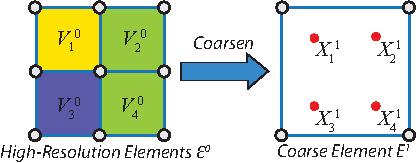
\includegraphics[width=0.6\textwidth]{images/coarseFine.pdf}
	\caption{The relationship between high-resolution and coarsened elements. At each quadrature point $\vr{X}_k^1$, the coarse element copies the corresponding energy density function $V_k^0$ from the high-resolution element.}
	\label{fig:coarseFine}
\end{figure}

We observe that even if the individual base material models are isotropic, the metamaterial can become anisotropic by assigning different material parameters at the quadrature points. We counter this by augmenting the metamaterial model with an anisotropic term, which improves fitting.
The complete model is then given by
\begin{align}
\begin{split}
V^1(\vr{u}^1, \, \vr{p}^1, \, C) &= \sum_{k=1}^8 \bigg( w_k \, V_k^0(\vr{u}^0, \,\vr{p}_k^1, \, \vr{X}_k^1)\\
& + C_k\left( \sqrt{\vr{v}^T\vr{F}_k^T\vr{F}_k\vr{v}} - 1\right)^2\bigg),\\
\label{eq:materialModel2}
\end{split}
\end{align}
where $\vr{v}$ is a unit-length direction of anisotropy and $C_k$ is the scaling parameter at the $k^{th}$ quadrature point. 

\subsection{Force Space Sampling}
\label{sec:force_space_sampling}
As mentioned previously, we take a sampling-based approach to metamaterial fitting. In order to fit our model (\autoref{eq:materialModel2}) to $V^0$ we first draw a number of samples from the deformation space of $\set{E}^0$ and compute $V^0$ for each sample.
If a user has prior knowledge of the set of meshes and simulations that they will require, then the best way to draw the samples is to run a number of anticipated simulations with various material combinations.
In this paper, we provide a more general method to draw samples for a metamaterial.
Initially, we attempted sampling by applying a random deformation to the corners of $\mathit{E}^1$; however, this led to many infeasible samples for very stiff materials.
In order to alleviate this problem we perform sampling in the force space.

For each element $\mathit{E}^0\in \, \set{E}^0$ we apply a set of randomly generated forces.
We solve an elastostatic problem to compute the deformation of $\set{E}^0$, using constraints to remove rigid motion. Recall that this is fast because $^0\set{E}$ consists of just 8 elements.
Each sample is then a tuple $\left\{\vr{u}^0, \, V^0\right\}$ (\autoref{fig:sampling}) where $^0\vr{u}$ are the nodal displacements of $^0\set{E}$, and $^0V$ is the strain energy density value of this deformed configuration.
\begin{figure}
	\centering
	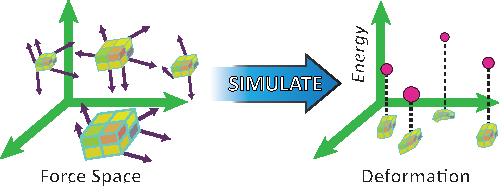
\includegraphics[width=0.6\columnwidth]{images/sampling.pdf}
	\caption{ We sample the energy function of a 2$\times$2$\times$2 block of hexahedra by applying random forces and deforming the block using FEM. Each set of forces results in a deformation-energy tuple which is used during fitting.}
	\label{fig:sampling}
\end{figure}

\subsection{Fitting}
\label{sec:fitting}
Given a set of deformation samples, $\left\{ \vr{u}^0, \,V^0\right\}$, we perform a least squares fit to determine the parameters, $\vr{p}^*$, for a given metamaterial (\autoref{fig:fitting}):
\begin{align}
\vr{p}^*= \underset{\vr{p}^1}{\operatorname{argmin}} \, \sum_{s=1}^{n_s}\left(V_s^0- \, V^1\left(\vr{r}\left(\vr{u}_s^0\right), \, \vr{p}^1\right)\right)^2,
\label{eq:fitting}
\end{align}
where $\vr{r}$ constructs $\vr{u}^1$ from $\vr{u}^0$, $n_s$ is the total number of samples, and $s$ indexes all samples. In our experiments we use the simplest form of $\vr{r}$ choosing it to extract the displacements of the corners of $\set{E}^0$.

\paragraph{Fitting in the Presence of Anisotropy}
If performed naively this optimization is nonlinear because we must simultaneously solve for $\vr{v}_k$, the preferred direction of anisotropy. This can severely slow the fitting procedure, especially in cases where it would otherwise be a linear least squares problem (i.e if all fine-scale materials are Neo-Hookean or a similarly simple material model).
To avoid this problem we first estimate all anisotropy directions, and then solve \autoref{eq:fitting} for the remaining material parameters.
Our intuition is that anisotropy manifests itself as preferential stretching along a particular axis. To find this axis, we apply stretching forces to a block in a discrete set of directions uniformly sampled over a sphere.
If the stretching force is close to the direction of anisotropy, then the amount of stretching deformation is reduced.
For any given stretching direction $\mathbf{v}$, we apply a stretching force and compute the deformation gradient $\mathbf{F}$ of  each quadrature point.
Under $\mathbf{F}$, a unit length vector in direction $\mathbf{v}$ is stretched to a new length $l = \|\mathbf{F}\mathbf{v}\|$.
The set of all 3D vectors $l\mathbf{v}$ forms an ellipse-like shape.
We find the principal axes of the ellipse (via SVD) and use them as directions of anisotropy.
\begin{figure}
	\centering
	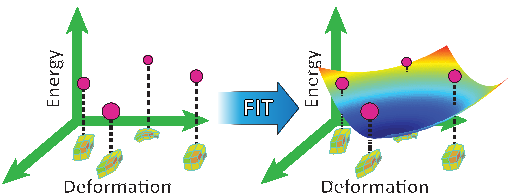
\includegraphics[width=0.6\columnwidth]{images/fitting.pdf}
	\caption{ Metamaterial potential energy functions are fitted to the deformation-energy samples using a least-squares optimization.}
	\label{fig:fitting}
\end{figure}
\paragraph{Regularization} Since vastly different material assignments, $^0\set{M}_k$, can produce the same metamaterial, our na\"{i}ve cost function (\autoref{eq:fitting}) can produce very large parameter values and even non-physical negative ones.
For example, consider a homogeneous material assignment at the high-resolution level.
The same metamaterial can be achieved by interleaving hard and soft materials at each fine element or by assigning a single, well chosen material to all fine elements.
To overcome this, we add a regularization term to control the parameter ranges and prevent overfitting of the training samples.
Our modified error function takes the following form:
\begin{equation}
\sum_{s=1}^{n_s}\left(V_s^0- \, V^1\left(\vr{r}\left(\vr{u}_s^0\right), \, \vr{p}^1\right)\right)^2 + 
\lambda\sum_k (\vr{p}_k^1 - \, \vr{p}_k^0)^2,
\end{equation}
which prevents material parameters from deviating too far from  $\set{M}_k^0$.
We chose the regularization constant $\lambda=0.02$ for the results in this paper.
In our experiments, since the base energy functions are linear with respect to the material parameters, the fitting problem can be solved by linear regression with regularization.

\begin{figure}
	\centering
	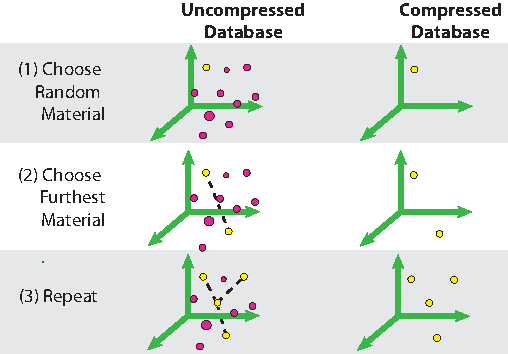
\includegraphics[width=0.6\columnwidth]{images/compression}
	\caption{Database compression step adds metamaterials to a compressed database by a farthest point sampling strategy.}
	\label{fig:compression}
\end{figure}

\subsection{Database Compression}
\label{sec:compression}
Given $n$ materials in the palette, the number of material combinations in a 2$\times$2$\times$2 block is $n^8$. In modern hardware, it is impossible to compute and store all material combinations even for a moderately-sized palette with $100$ materials.
In order to compress the number of materials stored in our metamaterial database, we select a small number of representative material combinations and remove all others. We compare materials in a feature space. In order to construct metamaterial feature vectors, we first select a common subset of deformations from all computed deformation samples. We then evaluate the potential energies of each metamaterial at each deformation sample. The stacked vector of energies becomes a metamaterial feature vector. 

Since our base materials differ in stiffness by orders of magnitude, we take the logarithm to measure the difference in ratio.
Let $D$ be the $L^2$ norm of log-energies between the two materials given by
\begin{equation}
D(A,B)=\sqrt{\sum_s (\log(V^{A}_{s})-\log(V^{B}_{s}))^2},
\end{equation} where $A$ and $B$ denote two distinct metamaterials in the database. 
Given the distance metric, we can select $k$ representatives materials using farthest point sampling~\cite{eldar1997farthest}. We randomly choose an initial metamaterial and then repeatedly select the material combination furthest away from any previous representatives -- continuing until we obtain $k$ representatives (\autoref{fig:compression}). This compression algorithm chooses $k$ samples that equally cover the metamaterial energy space, helping to preserve good behavior in our coarse simulations. 
\subsection{Hierarchical Coarsening}
While one level of coarsening can yield significant speed-ups, DDFEM can also be applied hierarchically.
As discussed in~\autoref{sec:compression}, the exponential growth of metamaterials palettes at each level makes it prohibitively expensive to perform fitting.
We address this by changing our coarsening strategy. 
Instead of choosing $\set{E}^0$ to be a 2$\times$2$\times$2 block we choose it to be a 2$\times$1$\times$1 block, which we coarsen. We construct an intermediate database of materials and compress. 
We then choose $\set{E}^0$ to be a 1$\times$2$\times$1 block, coarsen and compress, and finally a 1$\times$1$\times$2 block, coarsen and compress. Intermediate compression greatly reduces the number of samples we need to generate in order to populate the material parameter database for the next coarsening level. 
It is important to note that our intermediate databases only store lookup tables which allow us to extract appropriate material IDs for the next coarsening stage. Material parameters need only be stored in the final database since it is these elements that are simulated.
\begin{figure}
	\centering
	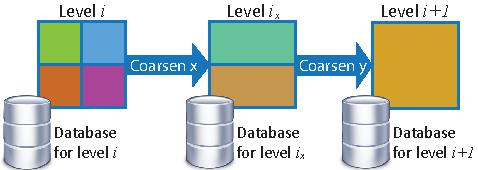
\includegraphics[width=0.7\textwidth]{images/hierchical}
	\caption{Hierarchical coarsening operates on one dimension at a time, performing clustering at each intermediate stage (here denoted $i_x$). This allows our compression algorithm to be applied aggressively, greatly reducing the number of energy samples we need for fitting material parameters. }
	\label{fig:hierarchy}
\end{figure}
\section{Runtime Simulation}
\label{sec:runtime}
Once our metamaterial database, $\set{P}^1$, has been constructed we can use it to perform fast online coarsening. 
Initially, the user loads geometry which is embedded in a hexahedral grid for simulation. Prior to simulation we iterate over all 2$\times$2$\times$2 blocks of hexahedral elements and perform mesh coarsening by replacing these 8 elements with a single coarse element. We perform a database lookup into $\set{P}^1$, using the material ID numbers of the 8 original elements, to quickly retrieve the optimal metamaterial for this coarse element. Database lookup is fast (even using our unoptimized, single-threaded implementation), and this is what makes DDFEM so appealing.
We achieve significant simulation speed-up from coarsening, retain accuracy in the simulation, and reduce the cost of material coarsening at runtime to a negligible amount.
	Our material model can be used in any simulation algorithm suitable for non-linear elasticity. In our experiments, we use Coin-IpOpt~\cite{ipopt} to implement static and dynamics simulations with tolerance (``tol'' option) set to $0.5$. We use Pardiso as our linear solver.
	For timing purposes, we limit Pardiso to single thread mode.
	The pseudo-code for static simulation is shown in \autoref{alg:sim}.
\begin{algorithm}
	\caption{Static Simulation}\label{alg:sim}
	\begin{algorithmic}[1]
		\REPEAT
		\STATE $\mathbf{f}$: global force vector
		\STATE $L$: triplet list for global stiffness matrix
		\FOR{each element e}
		\STATE compute elastic force $\mathbf{f}_e$
		\STATE add $\mathbf{f}_e$ to $\mathbf{f}$
		\ENDFOR
		\STATE add external force $\mathbf{f}_{ext}$ to $\mathbf{f}$
		\FOR{each element e}
		\STATE $\mathbf{K}_e$: element stiffness matrix
		\FOR{each quadrature point q}
		\STATE compute stiffness matrix $\mathbf{K}_q$ at quadrature point
		\STATE $\mathbf{K}_e+=\mathbf{K}_q$
		\ENDFOR
		\STATE append entries of $\mathbf{K}_e$ to $L$
		\ENDFOR
		\STATE sort $L$ to get sparse stiffness matrix $\mathbf{K}$
		\STATE set entries in $\mathbf{K}$ and $\mathbf{f}$ for fixed vertices
		\STATE $\Delta\mathbf{x}=\mathbf{K}^{-1}\mathbf{f}$
		\STATE compute step size $h$ using line-search
		\STATE $\mathbf{x}+=h\Delta\mathbf{x}$
		\UNTIL{convergence}
	\end{algorithmic}
\end{algorithm}

\begin{table}[!h]
	\centering
	\footnotesize
	\begin{tabular}{l c r r r r r r r r}
		\hline 
		\textbf{Example} &\textbf{grid size}&\textbf{rel sp}&\textbf{time/iter}&\textbf{iters}&\textbf{error}\\
		\hline
		{\color{HiResColor}Pushing(0)} &16$\times$16$\times$16&1.0 &1.010 &5&-\\
		{\color{DDFEMColor}Pushing(1)} &8$\times$8$\times$8   &11.5&0.087&5&8.91e-4\\
		{\color{DDFEMColor}Pushing(2)} &4$\times$4$\times$4   &31.4&0.032&5&1.36e-2\\
		\hline 
		{\color{HiResColor}Bending(0)} &8$\times$32$\times$8&1.0   &0.270 &28&-\\
		{\color{DDFEMColor}Bending(1)} &4$\times$16$\times$4&12.6  &0.028 & 22& 5.60e-2\\
		{\color{DDFEMColor}Bending(2)} &2$\times$8$\times$2 &22.7  &0.015 & 22&8.88e-2\\
		\hline 
		{\color{HiResColor}Twisting(0)} &8$\times$32$\times$8&1.0  & 0.300 & 16&-\\
		{\color{DDFEMColor}Twisting(1)} &4$\times$16$\times$4&15.2 & 0.031 & 10&1.56e-2\\
		{\color{DDFEMColor}Twisting(2)} &2$\times$8$\times$2 &20.7 & 0.019 & 12&3.28e-2\\
		\hline
		{\color{HiResColor}Buckling(0)} &128$\times$8$\times$16&1.0   &8.85 &32&-\\
		{\color{DDFEMColor}Buckling(1)} &64$\times$4$\times$8  &50.1 &0.28 &20&7.24e-3\\
		{\color{DDFEMColor}Buckling(2) }&32$\times$2$\times$4  &331.8&0.12 &7 &3.14e-2\\
		\hline
		{\color{HiResColor}Fibers(0)} &32$\times$100$\times$32&1.0  &193.85&17&-\\
		{\color{DDFEMColor}Fibers(1)} &16$\times$50$\times$16 &51.2 &4.95  &13& 2.94e-2\\
		{\color{DDFEMColor}Fibers(2)} &8$\times$25$\times$8   &489.5&0.96  &7 & 4.26e-2\\
		\hline
		{\color{HiResColor}Bridge(0)} &56177&1.0&43.44&14&-\\
		{\color{DDFEMColor}Bridge(1)} &9727&8.4&4.88&15&4.39e-3\\
		{\color{HiResColor}Bridge-arch(0)} &65684&1.0&54.99&3&-\\
		{\color{DDFEMColor}Bridge-arch(1)} &11695&8.1&7.84&3&3.68e-4\\
		\hline
		{\color{HiResColor}George(0)} &46152 & 1.0&52.19&23&-\\
		{\color{DDFEMColor}George(1)} &6755 & 16.4&3.49&21&2.86e-2\\
		{\color{HiResColor}George-bone(0)} &46152 & 1.0&41.35&12&-\\
		{\color{DDFEMColor}George-bone(1)} &6755 & 13.2&2.70&14&2.99e-2\\
		\hline
	\end{tabular}
	\vspace{-4pt}
	\caption{Relative performance, absolute performance in seconds and average vertex error relative to the bounding box size for full-resolution and coarsened simulations.
		Relative performance illustrates the performance increase gained by coarsening with respect to the time taken for the high-resolution static simulation to converge. Bracketed numbers after each example name indicate the number of coarsening levels with 0 indicating the {\color{HiResColor}high-resolution} simulation. All computation times are recorded using Coin-IpOpt running in single threaded mode on a 2.5 GHz Intel Core i7 processor. }
	\label{table:performance}
\end{table}
\begin{figure}[t]
	\centering
	\begin{tabularx}{0.92\columnwidth}{ Y Y }
		\textbf{Pushing} & \textbf{Twisting} \\
		\textbf{12x Faster} & \textbf{15x Faster}
	\end{tabularx}\\
	\subcaptionbox{}{
		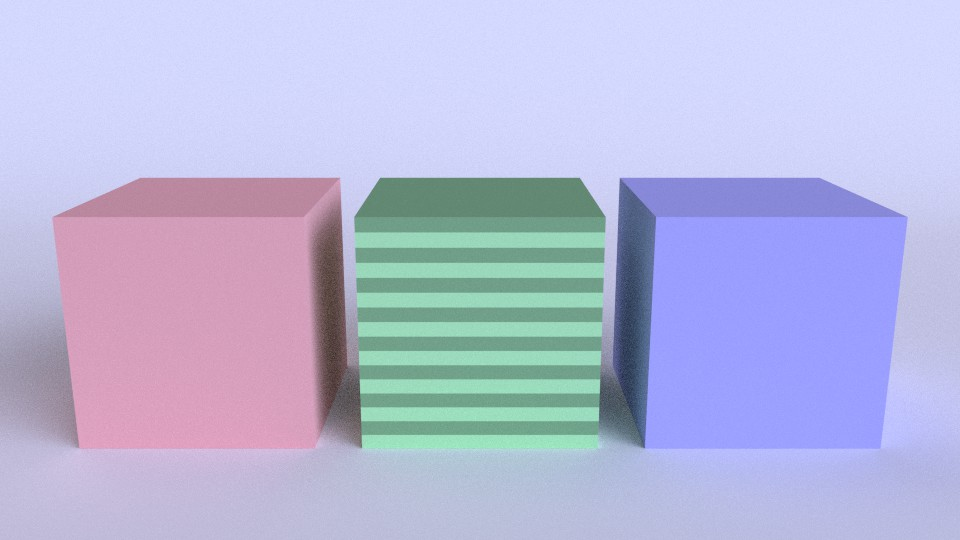
\includegraphics[width=0.45\textwidth]{images/push_l1_begin}
	}%\vrule
	\subcaptionbox{}{
		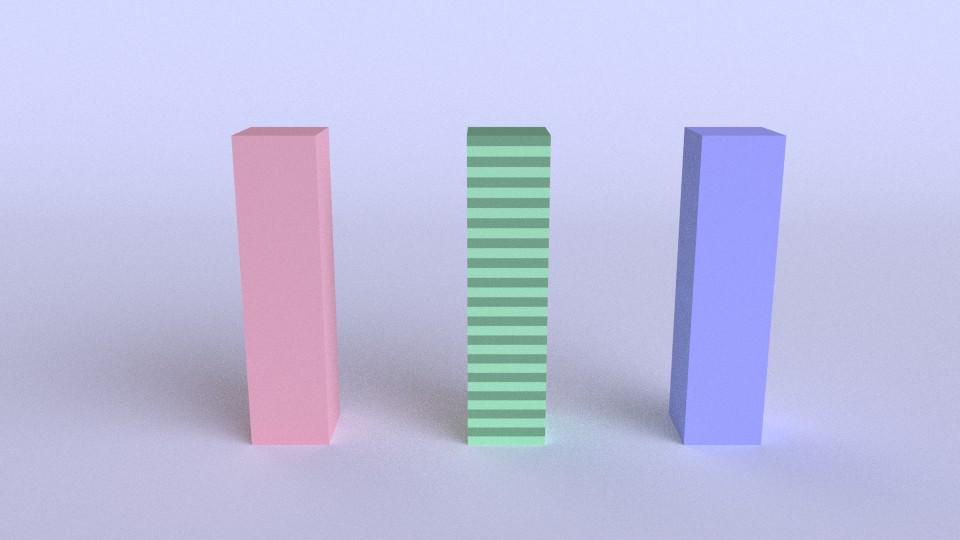
\includegraphics[width=0.45\textwidth]{images/twist_l1_begin}
	}
	\\
	\subcaptionbox{}{
		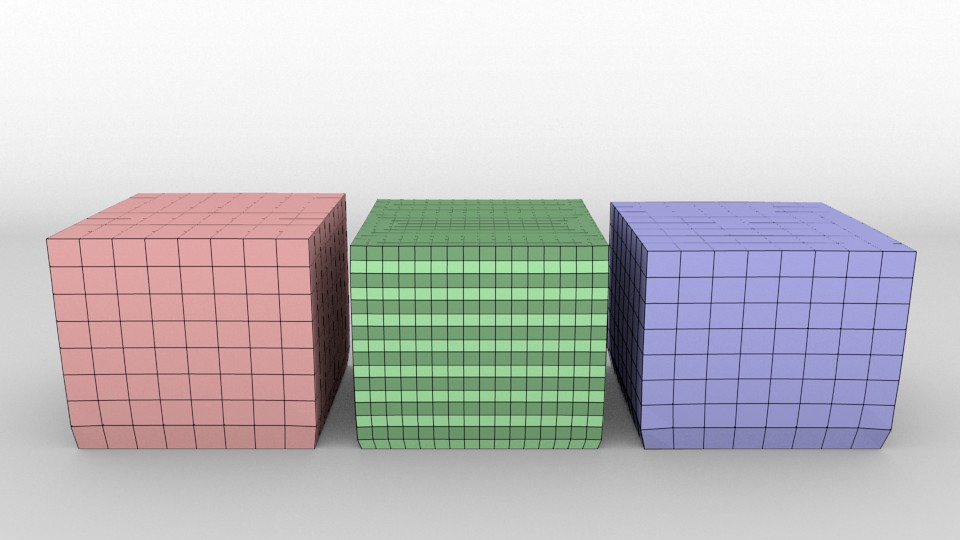
\includegraphics[width=0.45\textwidth]{images/push_l1_wire_end}
	}%\vrule
	\subcaptionbox{}{
		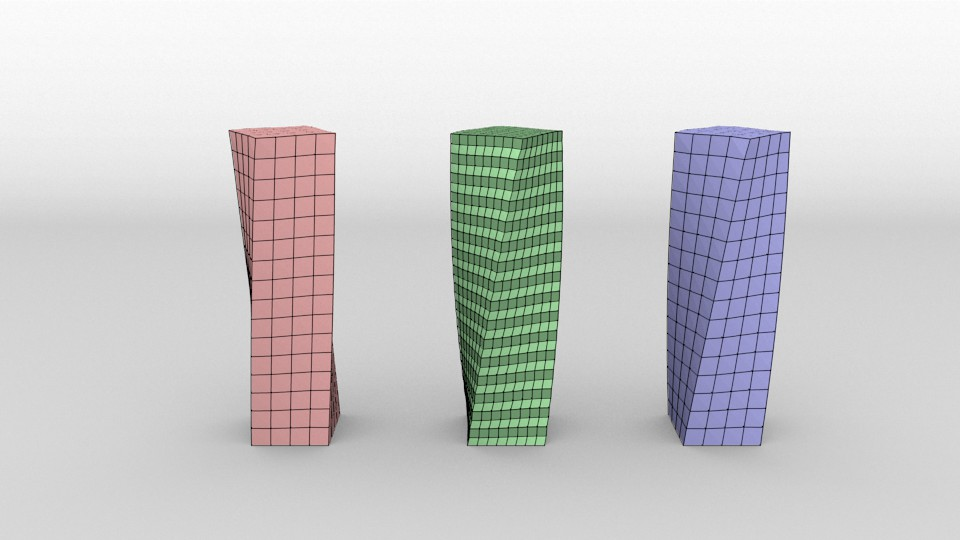
\includegraphics[width=0.45\textwidth]{images/twist_l1_wire_end}
	}
	%\vspace{-3mm}
	\caption{Examples of pushing a cube (a - Initial State, c - Compressed) and twisting a bar (b - Initial State, d - Compressed), both with heterogeneous material distribution. We compare {\DDFEM} to {\Naive} and the  ground-truth, {\HiRes}. We render wire frames to show the simulation meshes.}
	\label{fig:accuracy}
\end{figure}
\begin{figure}[t]
	\centering
	\begin{tabularx}{0.92\columnwidth}{ Y Y }
		\textbf{1 Level of Coarsening} & \textbf{\textbf{2 Levels of Coarsening}} \\
		\textbf{13x Faster} & \textbf{23x Faster}
	\end{tabularx}\\
	\subcaptionbox{}{
		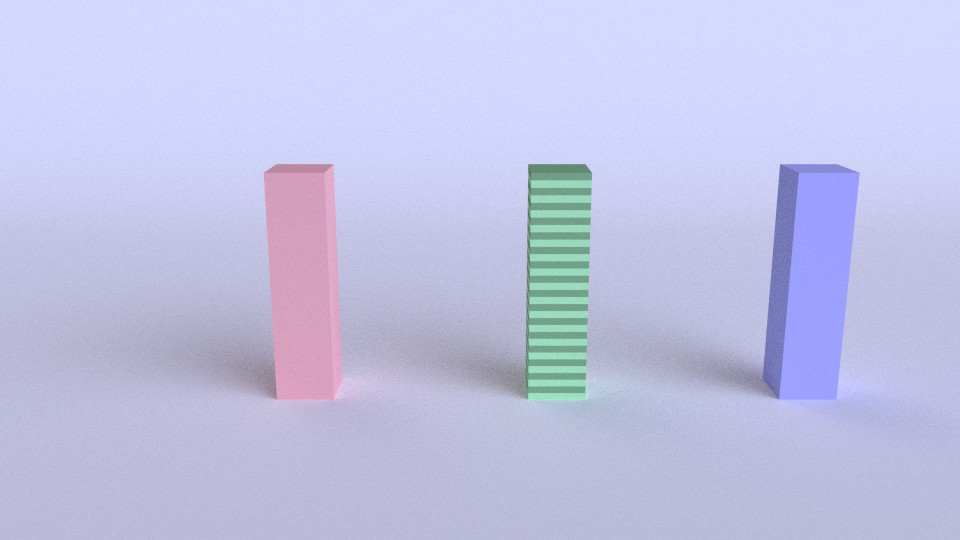
\includegraphics[width=0.47\columnwidth, trim=170px 105px 40px 105px, clip=true]{images/bend_l1_begin}
	}
	%\vrule
	\subcaptionbox{}{
		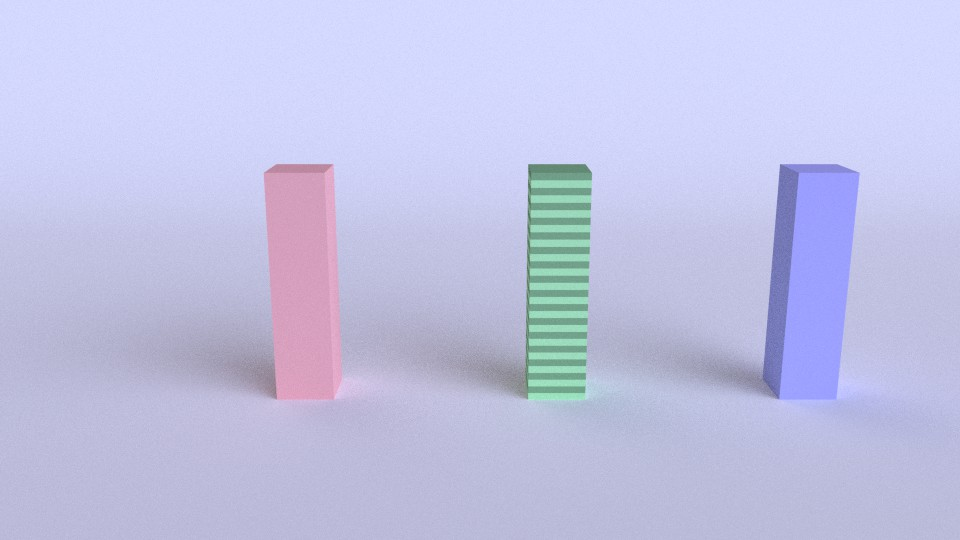
\includegraphics[width=0.47\columnwidth, trim=170px 105px 40px 105px, clip=true]{images/bend_l2_begin}
	}\\
	\subcaptionbox{}{
		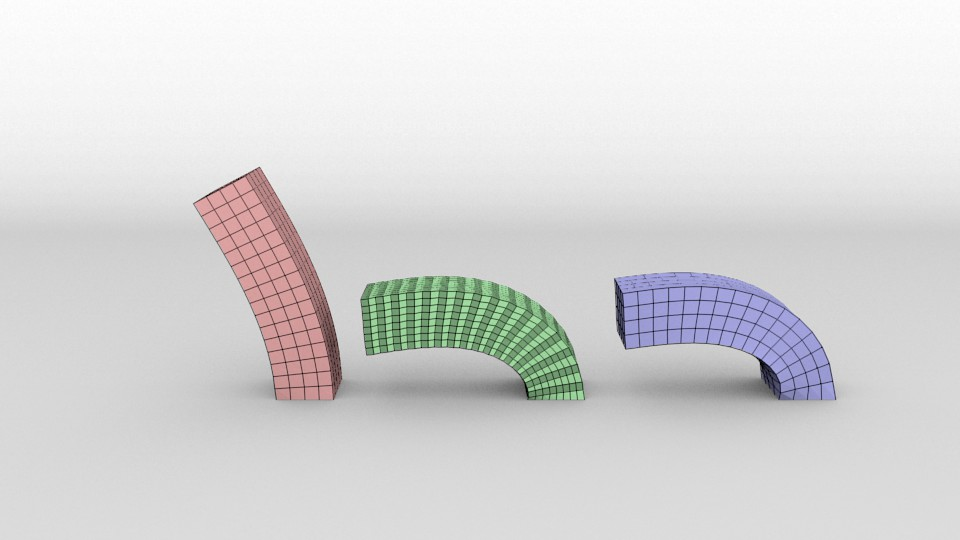
\includegraphics[width=0.47\columnwidth, trim=170px 105px 40px 105px, clip=true]{images/bend_l1_wire_end}
	}
	%\vrule
	\subcaptionbox{}{
		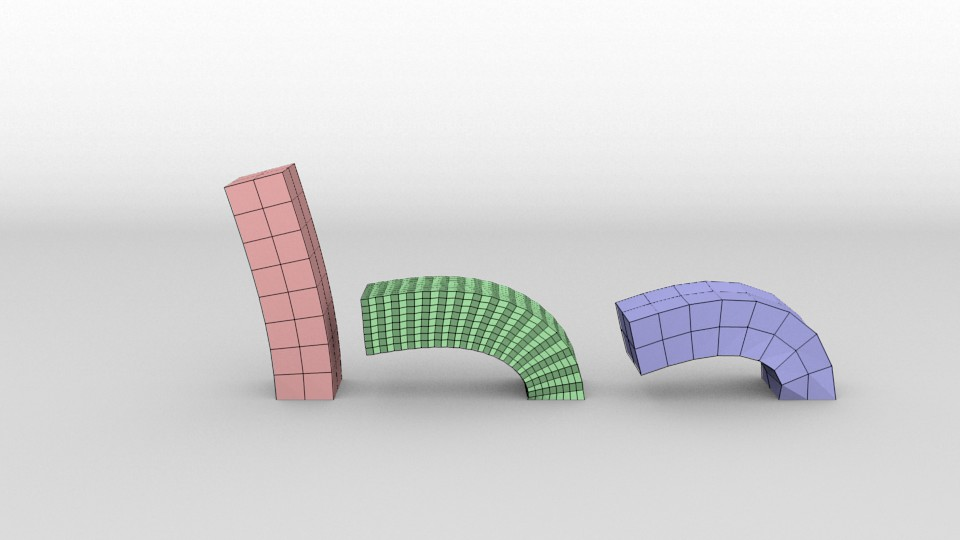
\includegraphics[width=0.47\columnwidth, trim=170px 105px 40px 105px, clip=true]{images/bend_l2_wire_end}
	}
	%\vspace{-8pt}
	\caption{Bending a heterogeneous bar: We compare {\DDFEM} to {\Naive} and a {\HiRes}. Subfigures (a, c) show comparison for 
		1 level of coarsening, and (b, d) show 2 levels of
		coarsening. The na\"{i}ve coarsening
		approach results in a much stiffer behavior, whereas our fitted
		model more closely approximates the fine model.}
	\label{fig:bending}
\end{figure}
\begin{figure}[t]
	\centering
	\begin{tabularx}{0.92\columnwidth}{ Y Y }
		\textbf{1 Level of Coarsening} & \textbf{\textbf{2 Levels of Coarsening}} \\
		\textbf{50x Faster} & \textbf{332x Faster}
	\end{tabularx}\\
	\subcaptionbox{}{
		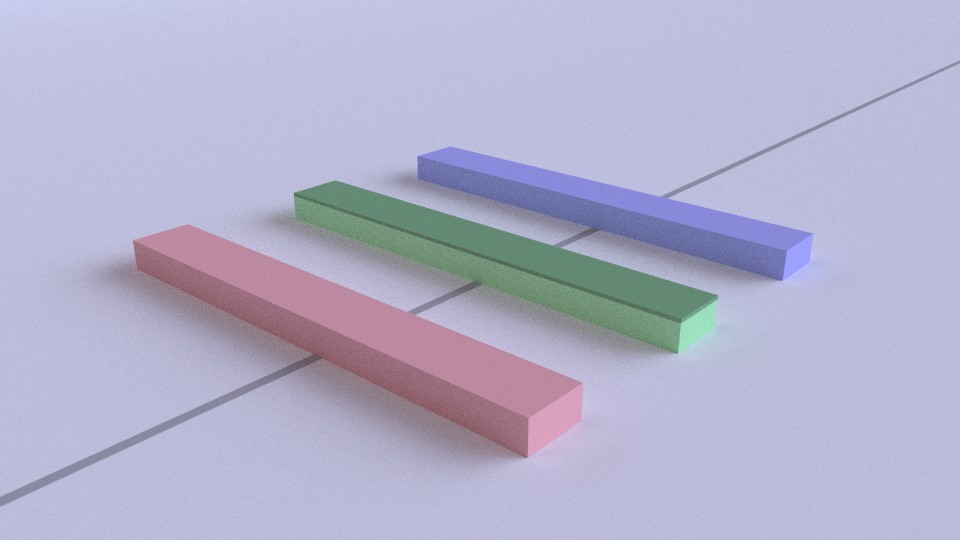
\includegraphics[width=0.47\columnwidth, trim=105px 60px 70px 115px, clip=true]{images/buckle_l1_begin}
	}%\vrule
	\subcaptionbox{}{
		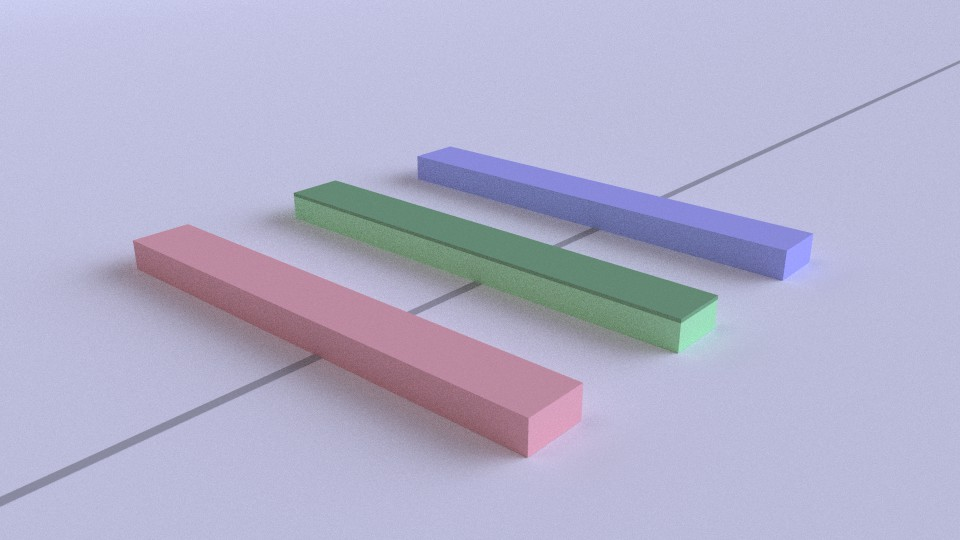
\includegraphics[width=0.47\columnwidth, trim=105px 60px 70px 115px, clip=true]{images/buckle_l2_begin}
	}
	\\
	\subcaptionbox{}{
		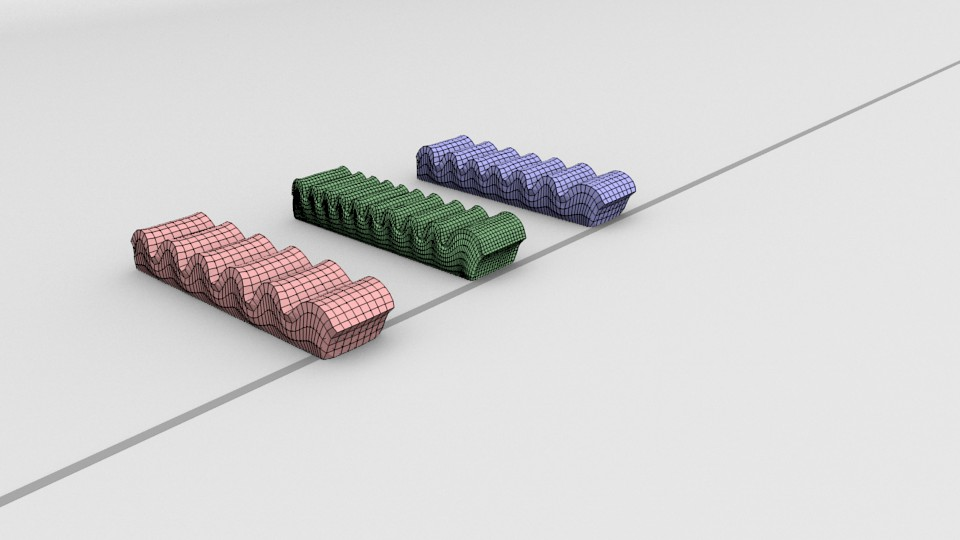
\includegraphics[width=0.47\columnwidth, trim=105px 60px 70px 115px, clip=true]{images/buckle_l1_wire_end}
	}
	%\vrule
	\subcaptionbox{}{
		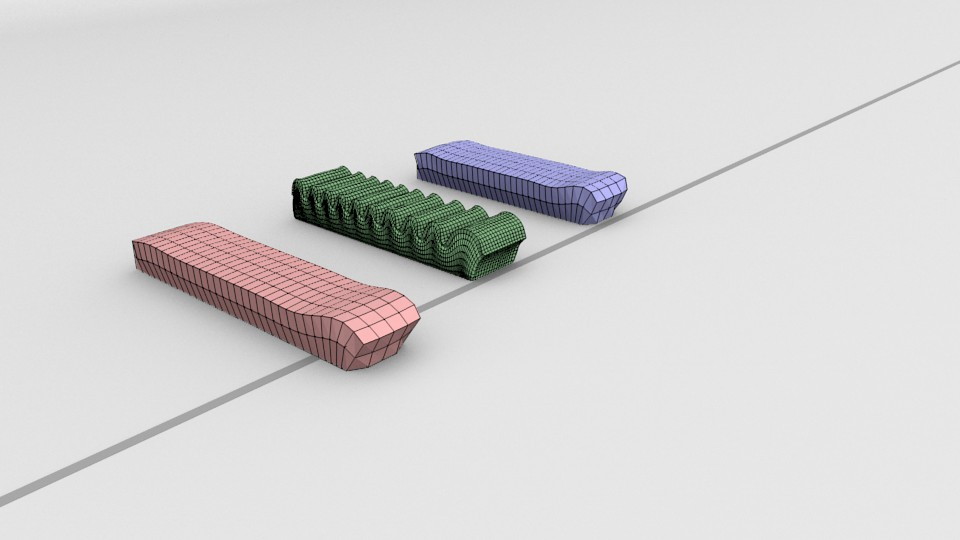
\includegraphics[width=0.47\columnwidth, trim=105px 60px 70px 115px, clip=true]{images/buckle_l2_wire_end}
	}
	\vspace{-2pt}
	\caption{Compressing a heterogeneous slab using {\Naive} (1 level and 2 levels of coarsening), {\DDFEM} (1 level and 2 levels of coarsening) and a {\HiRes}. The top, darker layer is stiffer, causing the object to buckle. The bottom vertices are constrained to stay on the floor. Figure (a,b) shows the slabs before compression, figure (c,d) shows the slabs after compression and figure. Notice that, after 1 level of coarsening, {\Naive} neither compresses nor buckles as much as either {\DDFEM} or {\HiRes}. After 2 levels of coarsening, \note{the buckling behavior is lost.}
		The {\Naive} fails to capture the compressive behavior of {\HiRes}, whereas {\DDFEM} does.}
	\label{fig:buckling}
\end{figure}
\begin{figure}
	\centering
	\begin{tabularx}{0.92\columnwidth}{ Y Y }
		\textbf{1 Level of Coarsening} & \textbf{\textbf{2 Levels of Coarsening}} \\
		\textbf{51x Faster} & \textbf{489x Faster}
	\end{tabularx}\\
	\subcaptionbox{}{
		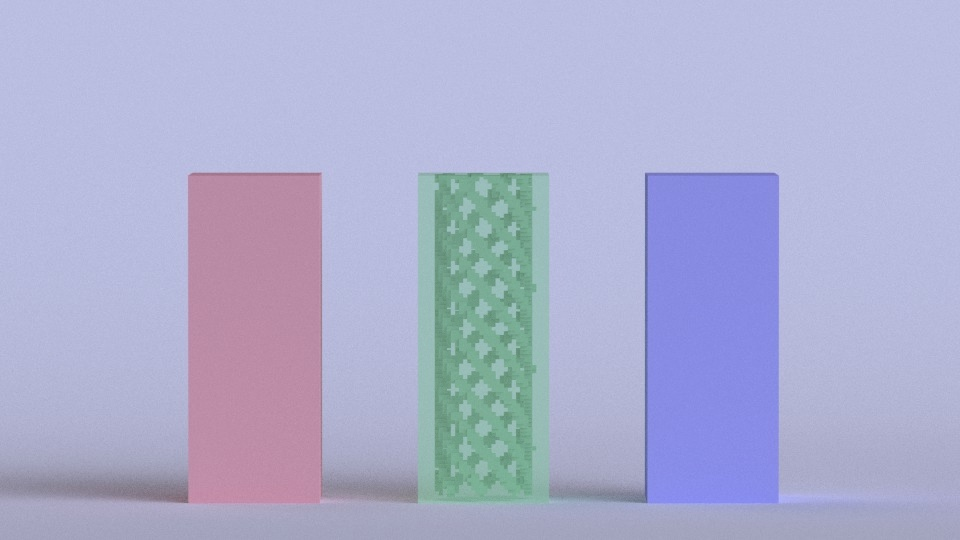
\includegraphics[width=0.4\textwidth]{images/fiber_l1_xray_begin}
	}%\vrule
	\subcaptionbox{}{
		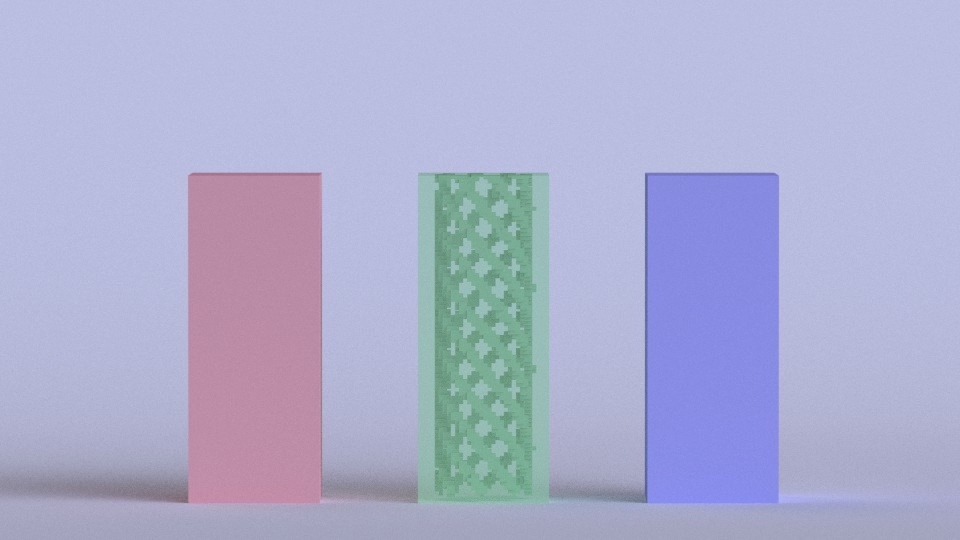
\includegraphics[width=0.4\textwidth]{images/fiber_l2_xray_begin}
	}  \\

	\subcaptionbox{}{
		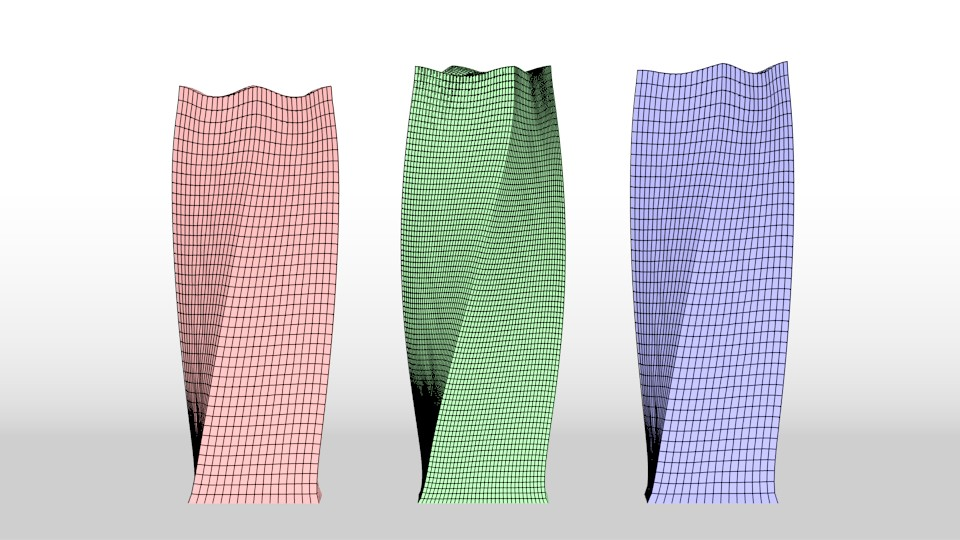
\includegraphics[width=0.4\textwidth]{images/fiber_l1_wire_end}
	}%\vrule
	\subcaptionbox{}{
		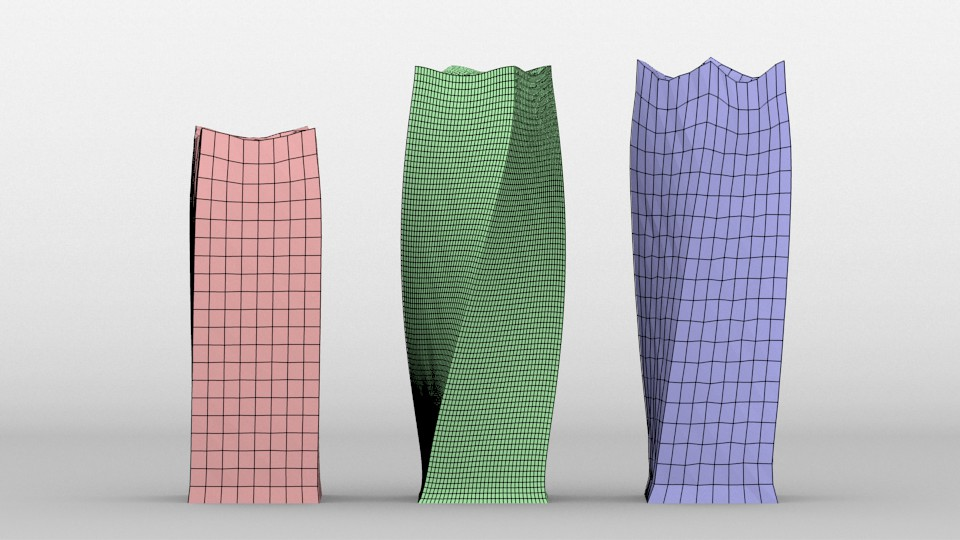
\includegraphics[width=0.4\textwidth]{images/fiber_l2_wire_end}
	}
	\vspace{-2pt}
	\caption{Simulating a bar with an embedded set of fibers using {\Naive}, {\DDFEM} and a {\HiRes}. Note that {\DDFEM} captures the characteristic twisting motion of the bar better than {\Naive}.  (a,b) shows the initial state of both bars while (c,d) shows the deformed state after pulling on the top of the bars.}
	\label{fig:fiberPull}
\end{figure}
\section{Results and Discussion}
\label{sec:result}
All the results shown here are simulated using nonlinear constitutive models at the fine scale. This and coarsening speed are the key differentiating factors between DDFEM and other coarsening algorithms such as~\citet{Nesme2009} and~\citet{Kharevych2009}.
\note{Our database starts with three Neo-hookean base materials with Young's modulus $1e5, 1e6, 1e7$ and Poisson's ration $0.45$. For comparison with 3D-printed objects, we used two base materials with measured Young's moduli.
	We use $500$ force directions, and sample $5$ magnitudes in each direction,
	resulting in $2500$ force samples for each material combination.
	In addition, we generate $500$ stretching samples for computing the direction of anisotropy. During fitting, we use shear modulus and Lam\'{e}'s first parameter,
	as well as the spring stiffness.
	We repeat the same process for the second level of coarsening, using
	$6561$ materials in the first level as base materials. We select
	$400$ representatives at each intermediate level.}

\subsection{Database}
One advantage of our compact metamaterial representation is the small amount of storage it requires. In fact we require only $6\times8=48$ floating-point values for each material at the first coarsening level and $6\times64=384$ values for the second level.
(For each finer element, $^0\vr{p}$ contains 2 material moduli plus $C, \vr{v}$.)
For further recursive levels, we can limit ourselves to $320$ values per material.
Our current 3 material database is $4$ megabytes in size.

\subsection{Simulation Results}
We show results from elastostatic simulations performed using DDFEM. We also demonstrate its performance advantages over high-resolution simulations. We render wire frames to show the discretizations of the high-resolution and coarse meshes. We first show examples of two simple simulations, the pushing and twisting of a rectangular object with heterogeneous, layered material distribution (\autoref{fig:accuracy}). Note that in all cases DDFEM qualitatively matches the behavior of the high-resolution simulation. We also compare the performance of DDFEM to a na\"{i}ve coarsening method that uses the material properties from 2$\times$2$\times$2 element blocks of the high-resolution simulation mesh at each corresponding quadrature point. \note{In our supplemental video we compare to a second baseline model which averages material parameters inside each coarse element. This average model is less accurate than the Na\"{i}ve model in all cases.} 

Na\"{i}ve approaches often exhibit pathological stiffness  for heterogeneous materials (illustrated by the lack of compression of the box and lack of twisting of the bar)~\cite{Nesme2009}. In these cases, DDFEM yields good speed ups while maintaining accuracy. For a single level of coarsening we achieve \emph{8 times or greater} speed ups for all examples. Performance numbers and mean errors are listed in \autoref{table:performance}.
Since the fine simulation and the coarse simulation have different numbers of vertices, we create a fine mesh from the coarse simulation by
trilinearly interpolating the fine vertices using the coarse displacements. The errors are measured by computing the average vertex distance relative
to the longest dimension of the bounding box in rest shape.
We also examine the behavior of DDFEM during bending (\autoref{fig:bending}). Yet again the na\"{i}ve coarsening method completely fails to capture the behavior of the high-resolution result, while DDFEM offers a much better approximation. 
\paragraph{Performance Analysis}
\note{\autoref{table:quadPerformance} shows time spent in quadrature evaluation versus in solver at coarse and fine levels.
	We use $8$ quadrature points for the first level of coarsening 
	and $64$ for the second level. The time for computing the local stiffness matrix for one element increases from $0.1$ms to $1$ms.
	In the second level, the speedup comes from the reduced number of elements over which to perform quadrature and the time required for the linear solver.
	
	To further investigate the performance of our coarsened simulations
	we replaced Pardiso with an assembly-free
	Jacobi-preconditioned conjugate gradient (CG) linear solver and used this to simulate our George-bone test case.
	While the overall runtime of the high-resolution simulation increased from $496$ to $2082$ seconds (most likely do to the unoptimized nature of our solver) our coarsened model achieved 20x and 67x speedups using one level and two levels of coarsening respectively. 
	One might expect no benefit from the second level of coarsening since the 
	number of quadrature points remains constant. 
	However, the number of CG iterations is roughly proportional to the number of vertices in the simulation mesh and thus the coarse model converges more quickly~(\autoref{fig:cg}).
	Since our  metamaterial models are not restricted to use
	a fixed number of quadrature points,
	one could design coarse models that are more tailored towards
	assembly-free solvers by reducing the number of quadrature points and simplifying the strain energy expressions.
}

\begin{figure}
	\centering
	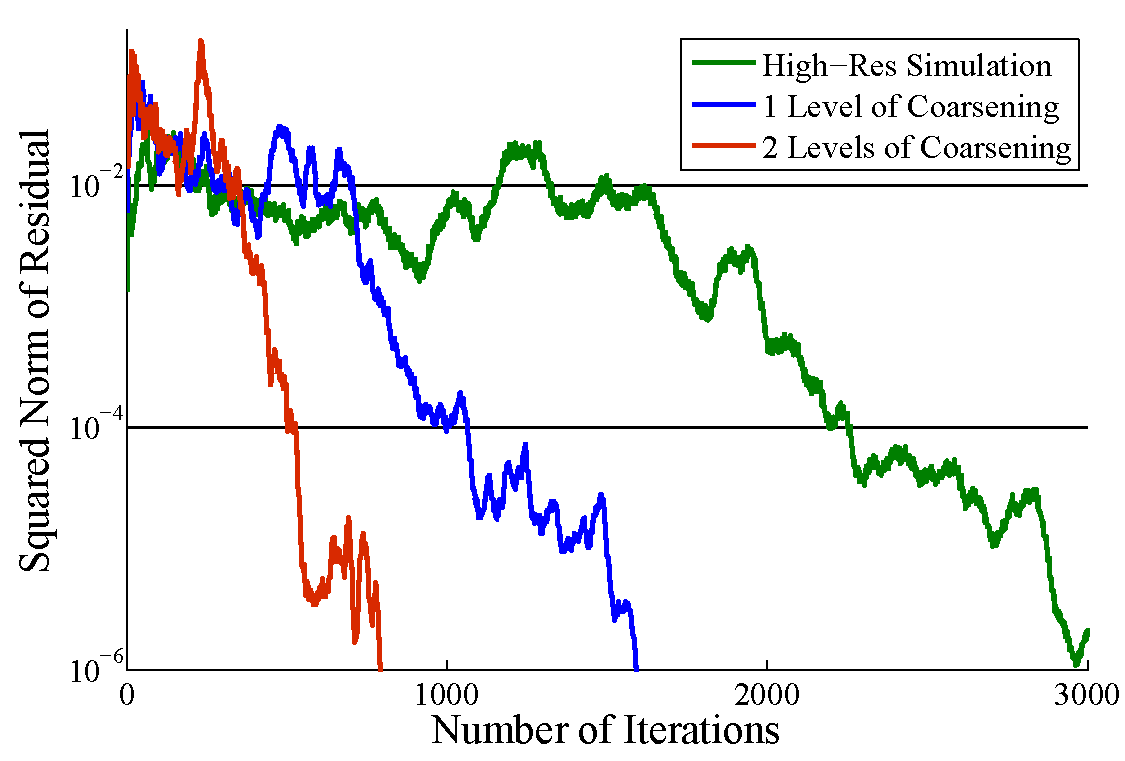
\includegraphics[width=0.6\textwidth]{figs/CGConverge.pdf}
	\caption{
		\note{Comparison of CG iterations on high-resolution and coarsened meshes of the George-bone example.
			The squared residual is measured as $\|\mathbf{K}\mathbf{x}-\mathbf{f}\|^2$.
			We observe that CG converges much faster on coarse meshes.
		}
	}\label{fig:cg}
\end{figure}

\begin{table}
	\centering
	\footnotesize
	\begin{tabular}{l c p{1cm} p{1cm} r }
		\hline 
		\textbf{Example} &\textbf{grid size}&\textbf{quad/iter} (12)&\textbf{time/iter} (2-21)&\textbf{iters}\\
		\hline 
		{\color{HiResColor}Bending(0)} &8$\times$32$\times$8   &  0.11  &0.27 &28\\
		{\color{DDFEMColor}Bending(1)} &4$\times$16$\times$4   &  0.015 &0.028&22\\
		{\color{DDFEMColor}Bending(2)} &2$\times$8$\times$2    &  0.014 &0.015&22\\
		\hline
		{\color{HiResColor}Buckling(0)} &128$\times$8$\times$16&  1.0   &8.8 &32\\
		{\color{DDFEMColor}Buckling(1)} &64$\times$4$\times$8  &  0.11  &0.28&20\\
		{\color{DDFEMColor}Buckling(2) }&32$\times$2$\times$4  &  0.10  &0.12&7\\
		\hline
		{\color{HiResColor}Fibers(0)} &32$\times$100$\times$32 & 10.0   &193&17\\
		{\color{DDFEMColor}Fibers(1)} &16$\times$50$\times$16  &  1.0   &4.9&13\\
		{\color{DDFEMColor}Fibers(2)} &8$\times$25$\times$8    &  0.68  &0.96&7\\
		\hline
	\end{tabular}
	\caption{\note{Portion of time in seconds used by quadrature computation during static simulation in seconds. Bracketed numbers indicate corresponding lines in Algorithm \ref{alg:sim}.}}
	\label{table:quadPerformance}
\end{table}
\paragraph{Complex material behavior} DDFEM can capture the gross behavior of  complex, spatially-varying material distributions. \autoref{fig:buckling} shows the results of applying DDFEM to a non-linearly elastic slab with a stiff ``skin.'' The bottom of the slab is constrained to slide along the ground with one end fixed. When force is applied to the free end of the slab, buckling occurs.  Somewhat obviously, DDFEM cannot replicate the frequency of the high-resolution buckling pattern due to the coarseness of the simulation mesh. However, it correctly captures the gross behavior of the bar and approximates the overall amount of compression well. \autoref{fig:buckling} also shows a comparison with 2nd level coarsening. In this case, the overall compression of the bar is still captured accurately. For this example DDFEM affords \emph{50 times} (1 level of coarsening) and \emph{332 times}  (2 levels of coarsening) performance improvements over the high-resolution simulation.  The artificial stiffness of the na\"{i}ve model can be seen in the reduced buckling and compression when compared to DDFEM at both coarsening levels.
%\vspace{-8pt}
\paragraph{Anisotropic material distribution} Next we explore the ability of DDFEM to handle highly anisotropic material distributions (\autoref{fig:fiberPull}). Specifically, we embed a helical set of stiff fibers in a soft, non-linearly elastic matrix. Pulling on the object induces a twisting. Again, at one coarsening level DDFEM captures this anisotropic behavior well, much better than the naive approach, and gains a \emph{51 times} speed up over the high-resolution simulation. Worth noting is that the DDFEM bar is slightly softer in the $y$-direction. This kind of inaccuracy should be expected. Since our method builds a low-dimensional approximation of a potential energy function we cannot hope to accurately reproduce the complete behavior of the high-resolution simulation.  What is important is that DDFEM captures the salient global behavior, in this case, the twisting of the bar. 
\paragraph{Geometry and material design} We present three examples of using DDFEM for geometry and material design. In the first example, we edit the material composition of the sole of a running shoe in order to stabilize it. \autoref{fig:shoe} shows the effect of the three material edits as well as relative speed up achieved over the full resolution simulation and coarsening time. DDFEM performance is always an order of magnitude more than that of the high-resolution simulation, and, most importantly, our coarsening times are on the order of milliseconds. We stress that our current implementation is completely single threaded and that coarsening, which in our case involves a simple database lookup, is inherently parallel.
In the second example, we add a supporting arch to a bridge. Prior to the addition of the support structure, the bridge sags catastrophically. The fast coarsening of DDFEM allows us to achieve an 8 fold increase in simulation performance using a single coarsening pass. In the third example, we add a rigid skeleton to a deformable character (George) in order  to control his pose. Here our single threaded, data-driven coarsening only takes ~200ms.  
\begin{figure*}
	\centering
	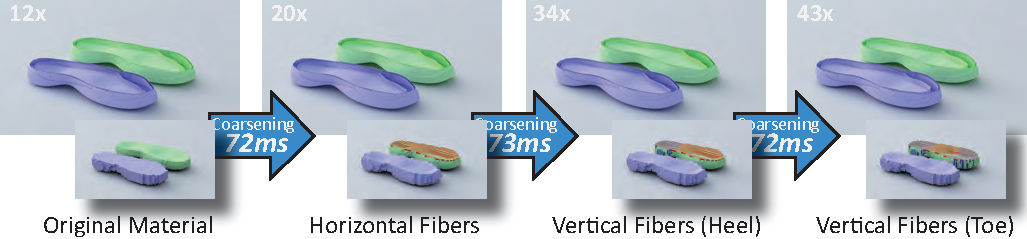
\includegraphics[width=0.90\textwidth]{images/DesignExampleShoe}
	\caption{Designing a shoe sole: We compare the performance of {\DDFEM} to that of {\HiRes} in the context of a material design problems. Large images show the effect of material changes on the sole of the shoe, which is being deformed under a ``foot-like'' pressure field. Inset images show the materials assigned to the shoe sole and the embedded finite element simulation mesh. Numbers within arrows show coarsening times between editing steps and the numbers in the upper left corner of each image show the relative performance of {\DDFEM} to  {\HiRes}. While the {\DDFEM} sole is made up of many metamaterials, we display it as a single color to distinguish it from the {\HiRes}.}
	\label{fig:shoe}
\end{figure*}

\begin{figure}
	\centering
	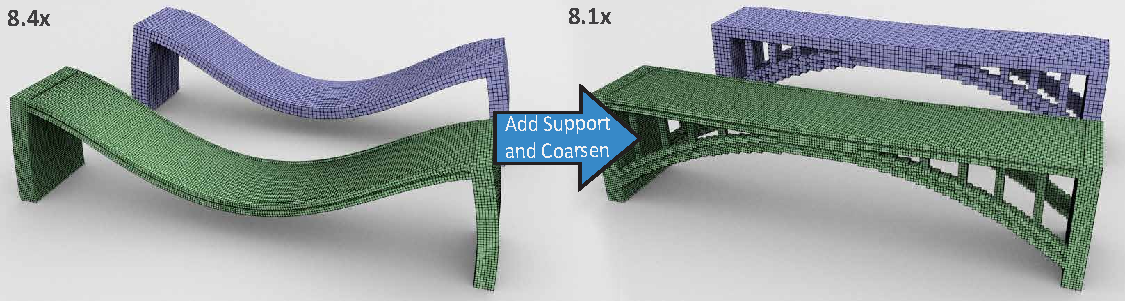
\includegraphics[width=0.8\textwidth]{images/bridge}
	\caption{Accelerating geometry change: We repair a structurally unsound bridge by adding a supporting arch (8x faster).}
	\label{fig:bridge}
\end{figure}
\begin{figure}
	\centering
	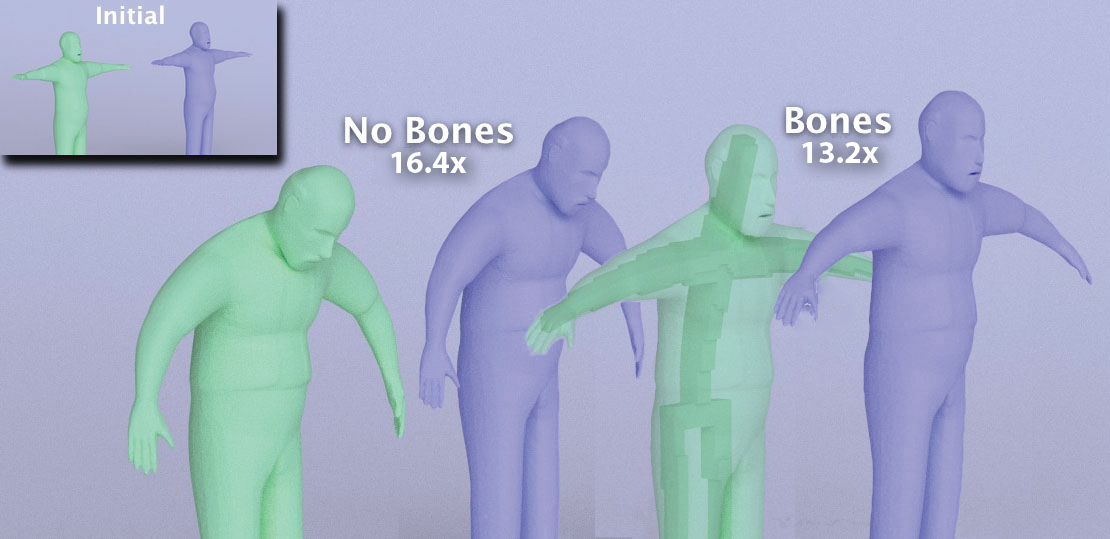
\includegraphics[width=0.8\textwidth]{images/georgeUpdate.png}
	\caption{Correcting George's posture using a rigid skeleton ({\HiRes} and {\DDFEM}).}
	\label{fig:george}
\end{figure}
\paragraph{Dynamics} Though the examples shown in this paper focus on static analysis, DDFEM is equally applicable to dynamic simulations. At its core, DDFEM simply supplies new, more accurate material models for use during simulation. This makes the method useful for accelerating various animation tasks as well. In the accompanying videos we show a dynamic simulation of our fiber embedded bar, computed using a standard linearly-implicit time integrator.

\begin{figure}
	\centering
	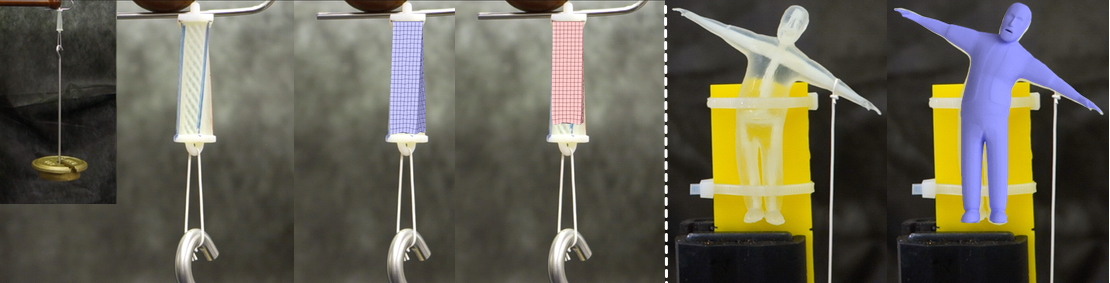
\includegraphics[width=0.8\textwidth]{images/experiments.jpg}
	\caption{A comparison of  {\DDFEM} (2 levels of coarsening) to real world deformations of 3D printed, multi-material designs. {\DDFEM} captures the twisting behavior of an anisotropic bar much more accurately than {\Naive}. Similarly {\DDFEM} accurately predicts the deformation of our heterogeneous George character. }
	\label{fig:experiments}
\end{figure}

\subsection{Fabricated Results}
Finally, we test the accuracy of our simulation against fabricated results, created using a Stratysys Object Connex 500 multimaterial 3D printer. We fabricated a bar with embedded helical fibers as well as our George character and applied specified loads to both. We show qualitative comparison of the deformed configurations of these real-world examples to our simulated results (\emph{2 levels of coarsening}-\autoref{fig:experiments}). Note that the simulation does an excellent job of predicting the deformed configuration of both objects.

\section{Limitations and Future Work}
Because DDFEM relies on a database compression step to combat the combinatorial explosion of metamaterials,  accuracy is heavily influenced by the set of representative metamaterials. Finding a better way to select metamaterial structures is an interesting area of future work.
Second, in our attempt to make our method geometry independent, some accuracy when dealing with partially filled boundary finite elements is sacrificed. Adding a parameterized boundary representation to the method, in order to more correctly handle non-axis aligned boundary conditions, could also be explored. Third, the method acts on discrete materials. While we believe that this is reasonable, considering the way that engineers and designers approach material design, a method that coarsens continuous spaces of non-linear materials could be beneficial.   

Many avenues of future work are promising. First, one could explore topologically aware meshing (i.e. in the same vein as~\citet{Nesme2009}) to allow better handling of models with large empty regions.
In fact shape function learning approaches, such as~\citet{Nesme2009} could be combined with our material learning approach to produce even more accurate simulations. Including these shape functions in our database could, for instance,  allow us to capture the wrinkles in our buckling example. Second, extending DDFEM to more complex material models, such as those involving plasticity, would be a useful exercise.
Third, DDFEM can be combined with an adaptive voxel grid as well as other dynamic meshing approaches to obtain further speed-ups.  Finally,  exploring hierarchical solvers based on DDFEM coarsening is a very attractive direction. Solvers such as multigrid methods rely on good coarse approximations to accelerate fine scale simulations. Using DDFEM for these approximations could improve the convergence rate, and thus the performance of such algorithms. 
